\documentclass[conference]{IEEEtran}
\usepackage{cite}
\usepackage{amsmath,amssymb,amsfonts}
\usepackage{graphicx}
\usepackage{textcomp}
\usepackage{xcolor}
\usepackage{booktabs}
\usepackage{multirow}
\usepackage{hyperref}
\usepackage[utf8]{inputenc}
\usepackage[T1]{fontenc}

\def\BibTeX{{\rm B\kern-.05em{\sc i\kern-.025em b}\kern-.08em
    T\kern-.1667em\lower.7ex\hbox{E}\kern-.125emX}}

\begin{document}

\title{Offensive Language Detection in Tamil Social Media Text Using Multilingual Transformers: A Comparative Study}

\author{
\IEEEauthorblockN{Author Name}
\IEEEauthorblockA{Department of Computer Science\\
University Name\\
City, Country\\
email@university.edu}
}

\maketitle

\begin{abstract}
The proliferation of offensive language on social media platforms poses a significant challenge, particularly in low-resource languages such as Tamil. While extensive research has been conducted on English offensive language detection, regional Indian languages remain critically underexplored. This paper presents a comparative study of three multilingual transformer models --- MuRIL, XLM-RoBERTa, and mBERT --- for detecting offensive language in Tamil and code-mixed Tamil-English (Tanglish) social media text. We fine-tune these models on the OffensEval Dravidian dataset (35,138 training samples across 6 classes) with inverse-frequency weighted loss to address severe class imbalance. Our experiments demonstrate that mBERT achieves the highest individual weighted F1-score of 0.7505, and a majority-voting ensemble further improves this to 0.7620, competitive with top-performing systems from the DravidianLangTech-2021 shared task. Contrary to expectations, Indian-language-specific pre-training (MuRIL) did not yield superior test-set performance. We further provide LIME-based explainability analysis to interpret model decisions and identify systematic failure patterns.
\end{abstract}

\begin{IEEEkeywords}
Offensive Language Detection, Tamil NLP, Multilingual Transformers, MuRIL, XLM-RoBERTa, Code-Mixed Text, Dravidian Languages
\end{IEEEkeywords}

%=====================================================
\section{Introduction}
%=====================================================

Social media platforms have become primary channels for public discourse, but they also serve as vectors for offensive content, cyberbullying, and targeted harassment. The rapid growth of internet usage in India --- with over 900 million users as of 2025 --- has led to a surge in user-generated content in regional languages, including Tamil, which is spoken by approximately 80 million people worldwide \cite{iamai2025}.

Despite the pressing need for automated content moderation in Indian languages, the overwhelming majority of offensive language detection research has focused on English \cite{fortuna2018survey}. This creates a critical gap: existing tools fail to detect offensive content in Tamil, particularly when expressed through code-mixing (switching between Tamil and English within a single sentence), transliteration (writing Tamil in Latin script, known as ``Tanglish''), and culturally specific expressions.

It is important to distinguish between \textit{hate speech} and \textit{offensive language} in this context. Hate speech specifically targets protected characteristics (race, religion, gender), while offensive language encompasses a broader category including profanity, insults, and targeted abuse \cite{davidson2017automated}. The OffensEval Dravidian dataset used in this study annotates \textit{offensive language}, which is a superset of hate speech.

Tamil social media text presents unique challenges for Natural Language Processing (NLP):

\begin{enumerate}
    \item \textbf{Code-mixing and Code-switching}: Users frequently alternate between Tamil and English within a single sentence (e.g., ``Padam vera level mass iruku'').
    \item \textbf{Script diversity}: Tamil content appears in Tamil Unicode script, Latin transliteration (Tanglish), or mixed scripts.
    \item \textbf{Non-standard orthography}: Social media Tamil lacks standardized spelling, with extensive abbreviations and phonetic spellings.
    \item \textbf{Cultural context dependency}: Caste references, fan community rivalries, and political slang carry connotations specific to Tamil culture.
\end{enumerate}

In this paper, we present a comparative study of three multilingual transformer models:

\begin{itemize}
    \item \textbf{MuRIL} (Multilingual Representations for Indian Languages) \cite{khanuja2021muril}: Pre-trained on 17 Indian languages including Tamil.
    \item \textbf{XLM-RoBERTa} \cite{conneau2020xlmr}: Trained on 100 languages from CommonCrawl.
    \item \textbf{mBERT} (Multilingual BERT) \cite{devlin2019bert}: The classic multilingual baseline trained on Wikipedia.
\end{itemize}

Our key contributions are:
\begin{enumerate}
    \item A systematic comparison of Indian-language-specific (MuRIL) vs.\ general multilingual (XLM-R, mBERT) pre-training for Tamil offensive language detection, with results contextualized against the DravidianLangTech-2021 shared task.
    \item A majority-voting ensemble strategy that improves over the best individual model.
    \item LIME-based explainability analysis with concrete word-level attribution examples.
    \item Identification of systematic error patterns and actionable recommendations.
\end{enumerate}

%=====================================================
\section{Related Work}
%=====================================================

\subsection{Offensive Language Detection in English}

Early offensive language detection relied on traditional machine learning using TF-IDF features with SVM classifiers \cite{waseem2016hateful}. Deep learning brought significant improvements with CNN and LSTM architectures \cite{badjatiya2017deep}. The transformer revolution, initiated by BERT \cite{devlin2019bert}, established new benchmarks. Davidson et al.\ \cite{davidson2017automated} highlighted the important distinction between hate speech and general offensive language, showing that even human annotators struggle with the boundary. HateBERT \cite{caselli2021hatebert} demonstrated the value of domain-specific pre-training.

\subsection{Multilingual and Cross-lingual Approaches}

Multilingual models such as mBERT \cite{devlin2019bert} and XLM-RoBERTa \cite{conneau2020xlmr} enable zero-shot cross-lingual transfer. However, performance drops significantly for low-resource and code-mixed text \cite{pamungkas2019cross}. MuRIL \cite{khanuja2021muril} addresses this by incorporating transliterated and romanized Indian-language text during pre-training.

\subsection{Offensive Language Detection in Dravidian Languages}

The DravidianLangTech shared tasks \cite{chakravarthi2021dravidian} catalyzed research in Tamil, Malayalam, and Kannada. The shared task attracted over 30 participating teams, with winning systems achieving weighted F1-scores in the 0.75--0.78 range for Tamil \cite{chakravarthi2021dravidian}. Top approaches included ensemble methods combining transformers with traditional features \cite{dowlagar2021cfilt}, data augmentation for class imbalance \cite{risch2020data}, and multi-task learning \cite{rajamanickam2020joint}. However, systematic comparisons coupled with explainability analysis remain limited.

\subsection{Explainable AI for Offensive Language}

Explainability is critical for building trust in automated moderation. LIME \cite{ribeiro2016lime} and SHAP \cite{lundberg2017shap} provide model-agnostic explanations. HateXplain \cite{mathew2021hatexplain} demonstrated that models sometimes rely on spurious correlations rather than genuine offensive indicators. Our work applies LIME specifically to code-mixed Tamil text, revealing unique challenges.

%=====================================================
\section{Dataset}
%=====================================================

\subsection{OffensEval Dravidian Dataset}

We use the Tamil configuration of the OffensEval Dravidian dataset \cite{chakravarthi2021dataset}, sourced from YouTube comments. The original dataset provides train and validation splits. Following standard practice, we split the original validation set 50--50 into our validation and test sets, as the official shared task test set labels are not publicly available.

\begin{table}[!t]
\centering
\caption{Dataset Split Statistics}
\label{tab:dataset}
\begin{tabular}{lr}
\toprule
\textbf{Split} & \textbf{Samples} \\
\midrule
Train & 35,138 \\
Validation & 2,194 \\
Test & 2,194 \\
\midrule
\textbf{Total} & \textbf{39,526} \\
\bottomrule
\end{tabular}
\end{table}

\textbf{Note:} Since we use a custom test split rather than the official shared task test set, our results are not directly comparable with shared task leaderboard scores. We include shared task results in Table~\ref{tab:baselines} for approximate context only.

\subsection{Label Taxonomy and Distribution}

The dataset employs a 6-class taxonomy with severe class imbalance, as shown in Table~\ref{tab:labels} and Fig.~\ref{fig:label_dist}. The \texttt{Not\_offensive} class comprises 72.4\% of all samples, while \texttt{Offensive\_Targeted\_Other} constitutes only 1.3\%.

\begin{table}[!t]
\centering
\caption{Label Distribution (Training Set)}
\label{tab:labels}
\begin{tabular}{lrr}
\toprule
\textbf{Label} & \textbf{Count} & \textbf{\%} \\
\midrule
Not\_offensive & 25,424 & 72.4 \\
Offensive\_Untargeted & 2,906 & 8.3 \\
Offensive\_Targeted\_Group & 2,557 & 7.3 \\
Offensive\_Targeted\_Individual & 2,343 & 6.7 \\
not-Tamil & 1,454 & 4.1 \\
Offensive\_Targeted\_Other & 454 & 1.3 \\
\bottomrule
\end{tabular}
\end{table}

\begin{figure}[!t]
\centering
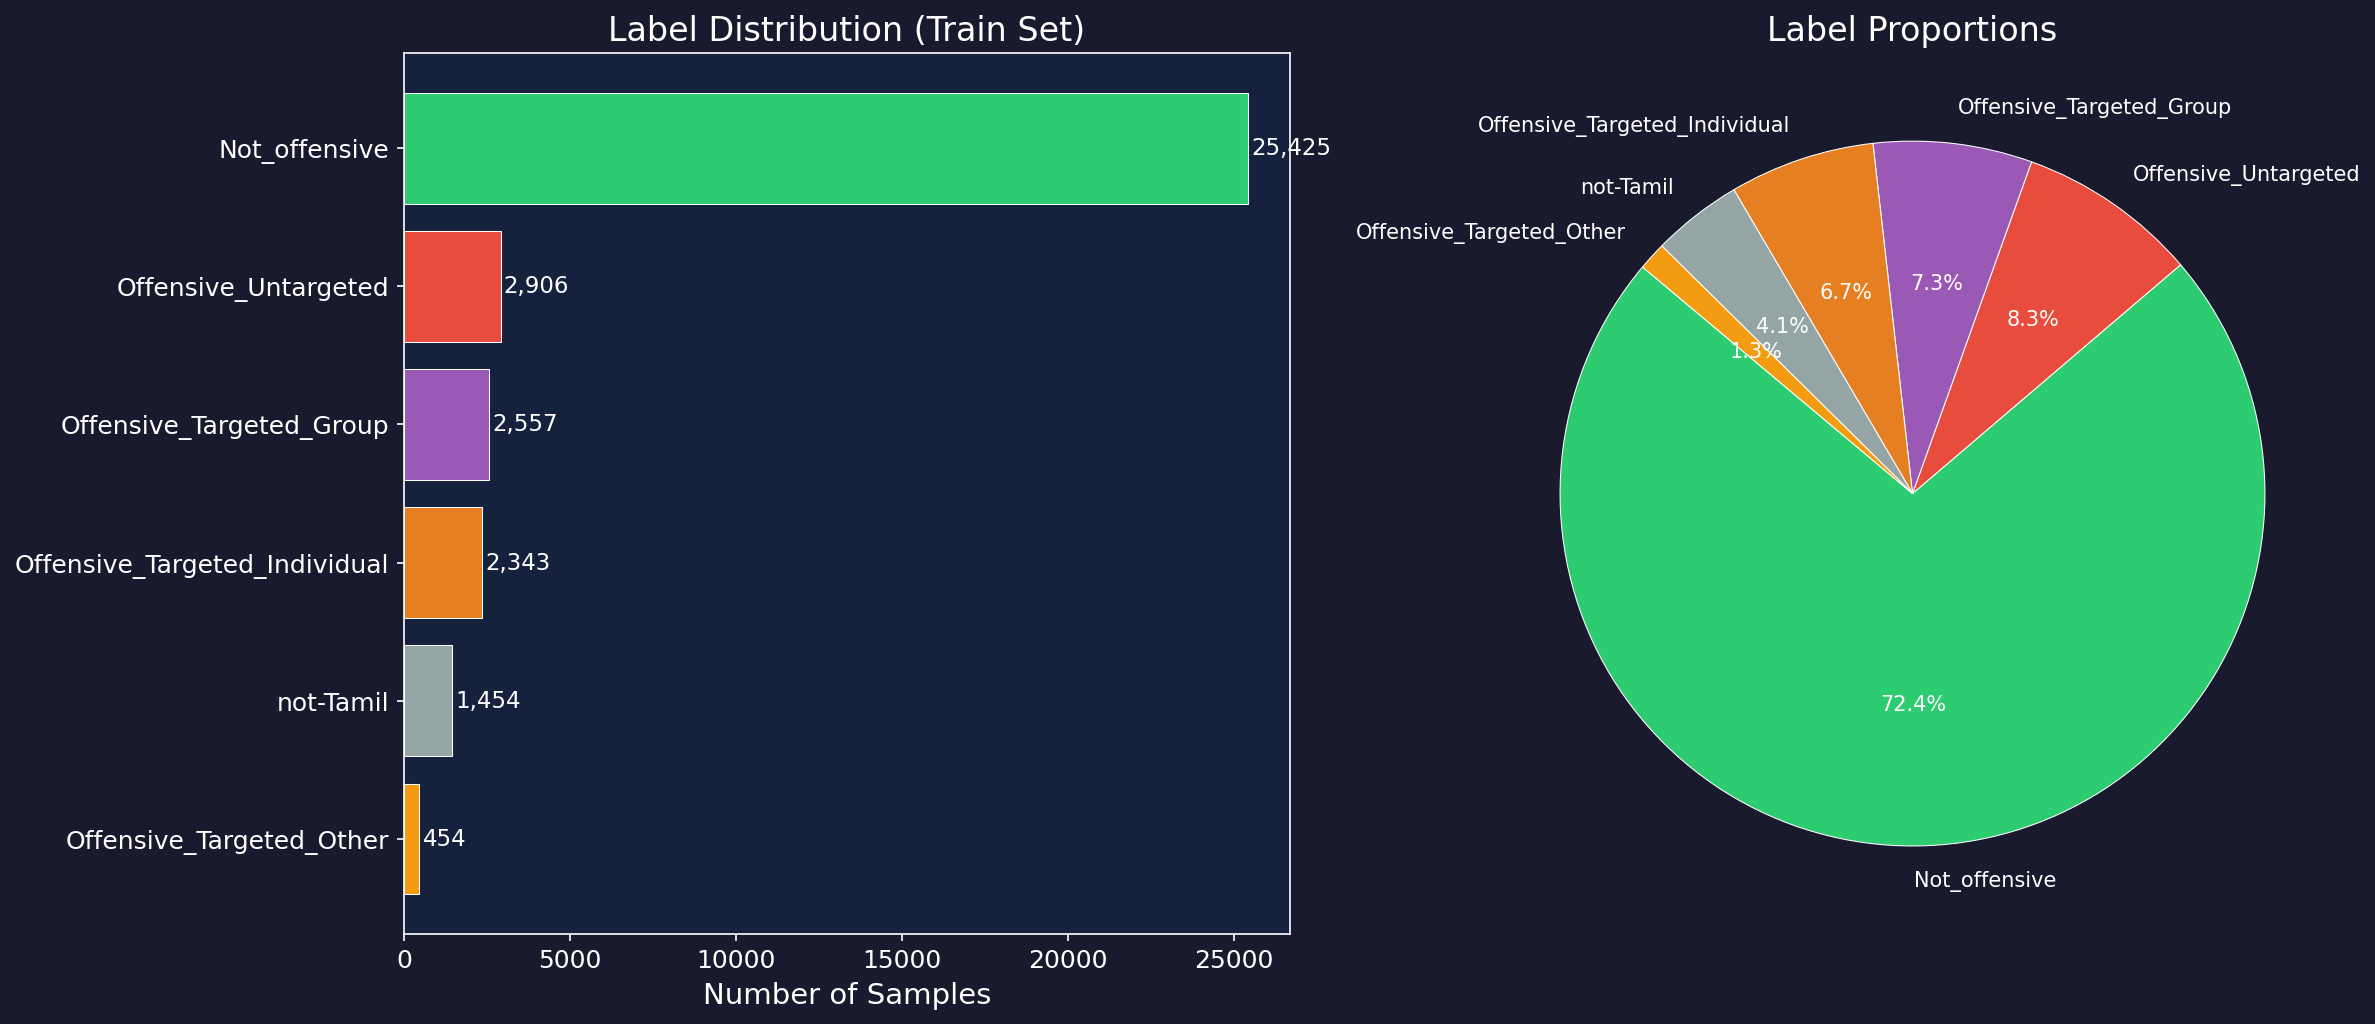
\includegraphics[width=0.95\columnwidth]{figures/label_distribution.png}
\caption{Label distribution in the training set, showing severe class imbalance.}
\label{fig:label_dist}
\end{figure}

\subsection{Script Analysis}

The dataset contains three script categories: Latin/Tanglish (81.2\%), Tamil Unicode (17.6\%), and code-switched mixed-script (1.1\%). The dominance of Latin-script content reflects the prevalence of transliterated Tamil on social media. Note that the ``Latin'' category includes both transliterated Tamil (Tanglish) and pure English comments; we do not distinguish between these sub-categories in our preprocessing.

%=====================================================
\section{Methodology}
%=====================================================

Fig.~\ref{fig:architecture} presents an overview of our pipeline.

\begin{figure*}[!t]
\centering
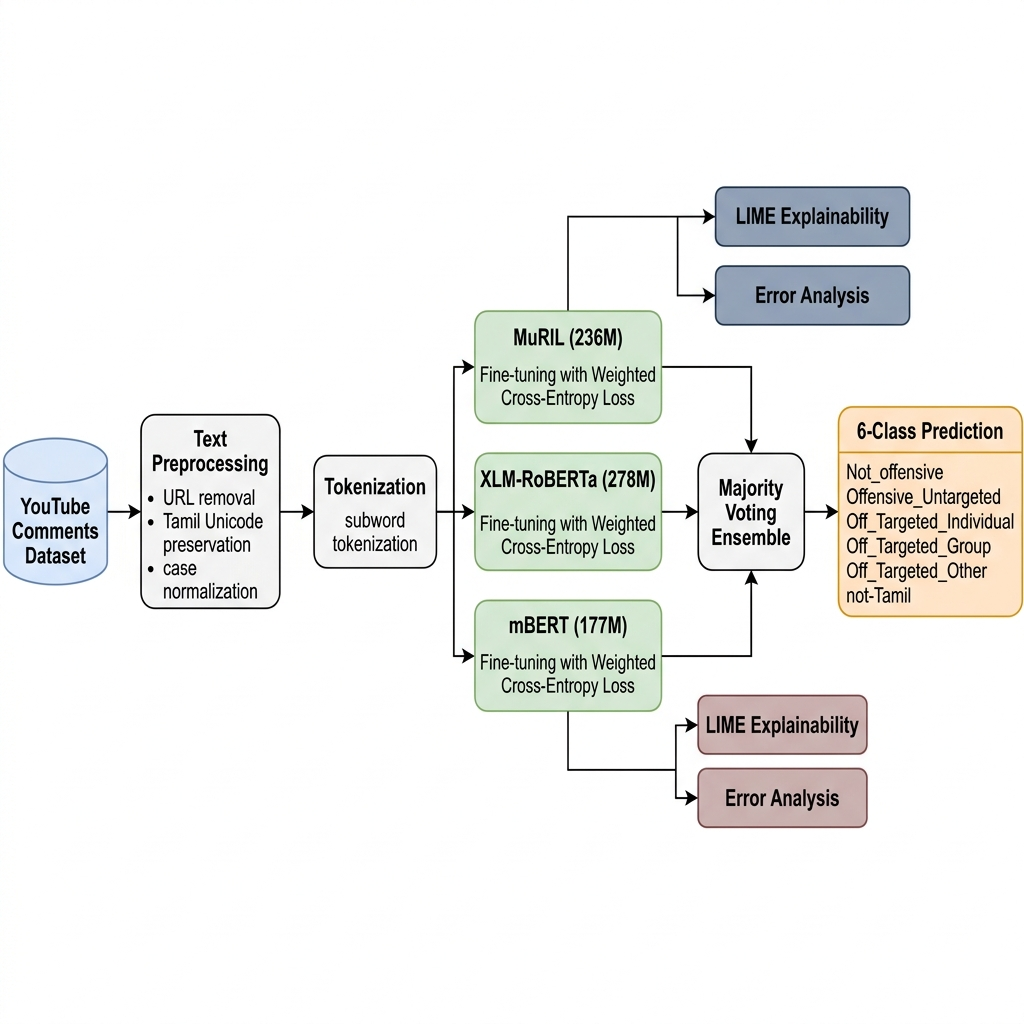
\includegraphics[width=0.85\textwidth]{figures/architecture.png}
\caption{System architecture. YouTube comments are preprocessed, tokenized, and fed into three parallel transformer models fine-tuned with weighted cross-entropy loss. Predictions are combined via majority-voting ensemble. LIME analysis is performed on the best individual model.}
\label{fig:architecture}
\end{figure*}

\subsection{Text Preprocessing}

We apply: (1) URL and @mention removal, (2) hashtag symbol removal (text preserved), (3) non-alphanumeric character filtering with Tamil Unicode range (U+0B80--U+0BFF) preservation, (4) Latin case normalization, and (5) whitespace normalization. We do not apply stemming or lemmatization, as these tools are limited for Tamil.

\subsection{Model Architectures}

Table~\ref{tab:models} summarizes the three models. MuRIL includes transliterated/romanized text in its pre-training data, directly addressing Tanglish-dominant input.

\begin{table}[!t]
\centering
\caption{Model Specifications}
\label{tab:models}
\begin{tabular}{lccc}
\toprule
\textbf{Model} & \textbf{Params} & \textbf{Langs} & \textbf{Pre-training Data} \\
\midrule
MuRIL & 236M & 17 & Indian web + transliterations \\
XLM-R & 278M & 100 & CommonCrawl (2.5TB) \\
mBERT & 177M & 104 & Wikipedia \\
\bottomrule
\end{tabular}
\end{table}

\subsection{Training Configuration}

All models are fine-tuned with: learning rate $2 \times 10^{-5}$, effective batch size 32, max sequence length 128, 5 epochs with early stopping patience 2, weight decay 0.01, warmup ratio 0.1, AdamW optimizer, FP16 mixed precision, and weighted F1-score for model selection. Training was performed on a single NVIDIA Tesla T4 GPU via Google Colab.

\textbf{Limitation:} All experiments use a single random seed. Results may vary with different seeds; we acknowledge this as a threat to external validity. Multi-seed experiments with confidence intervals are planned as future work.

\subsection{Class Imbalance Handling}

We employ inverse-frequency class weighting:

\begin{equation}
w_c = \frac{N}{C \times n_c}
\end{equation}

where $N$ = total samples, $C$ = number of classes, $n_c$ = count of class $c$. This produces weights ranging from $\approx$1.0 (Not\_offensive) to $\approx$12.9 (Offensive\_Targeted\_Other).

\subsection{Ensemble Strategy}

We combine all three models' predictions via majority voting. For each test sample, the class predicted by at least 2 of 3 models is selected. This requires no additional training.

%=====================================================
\section{Results}
%=====================================================

\subsection{Overall Performance}

\begin{table}[!t]
\centering
\caption{Model Comparison on Test Set}
\label{tab:results}
\begin{tabular}{lccccc}
\toprule
\textbf{Model} & \textbf{Acc.} & \textbf{F1-W} & \textbf{F1-M} & \textbf{Prec-W} & \textbf{Rec-W} \\
\midrule
MuRIL & 0.7115 & 0.7310 & 0.4405 & 0.7637 & 0.7115 \\
XLM-R & 0.7019 & 0.7275 & 0.4743 & 0.7791 & 0.7019 \\
mBERT & 0.7288 & 0.7505 & \textbf{0.4972} & 0.7840 & 0.7288 \\
\midrule
Ensemble & \textbf{0.7502} & \textbf{0.7620} & 0.4947 & \textbf{0.7817} & \textbf{0.7502} \\
\bottomrule
\end{tabular}
\end{table}

Table~\ref{tab:results} presents the results. mBERT achieves the best individual F1-W (0.7505). The ensemble improves F1-W to 0.7620 (+1.15\% absolute) but slightly decreases F1-Macro (0.4947 vs.\ 0.4972). This trade-off is expected: majority voting favors the majority class, improving weighted metrics at the cost of minority-class macro performance.

Notably, mBERT outperforms MuRIL on the test set despite MuRIL achieving the highest validation F1 during training (0.7309 vs.\ 0.7322), as shown in Fig.~\ref{fig:training_analysis}.

\begin{figure}[!t]
\centering
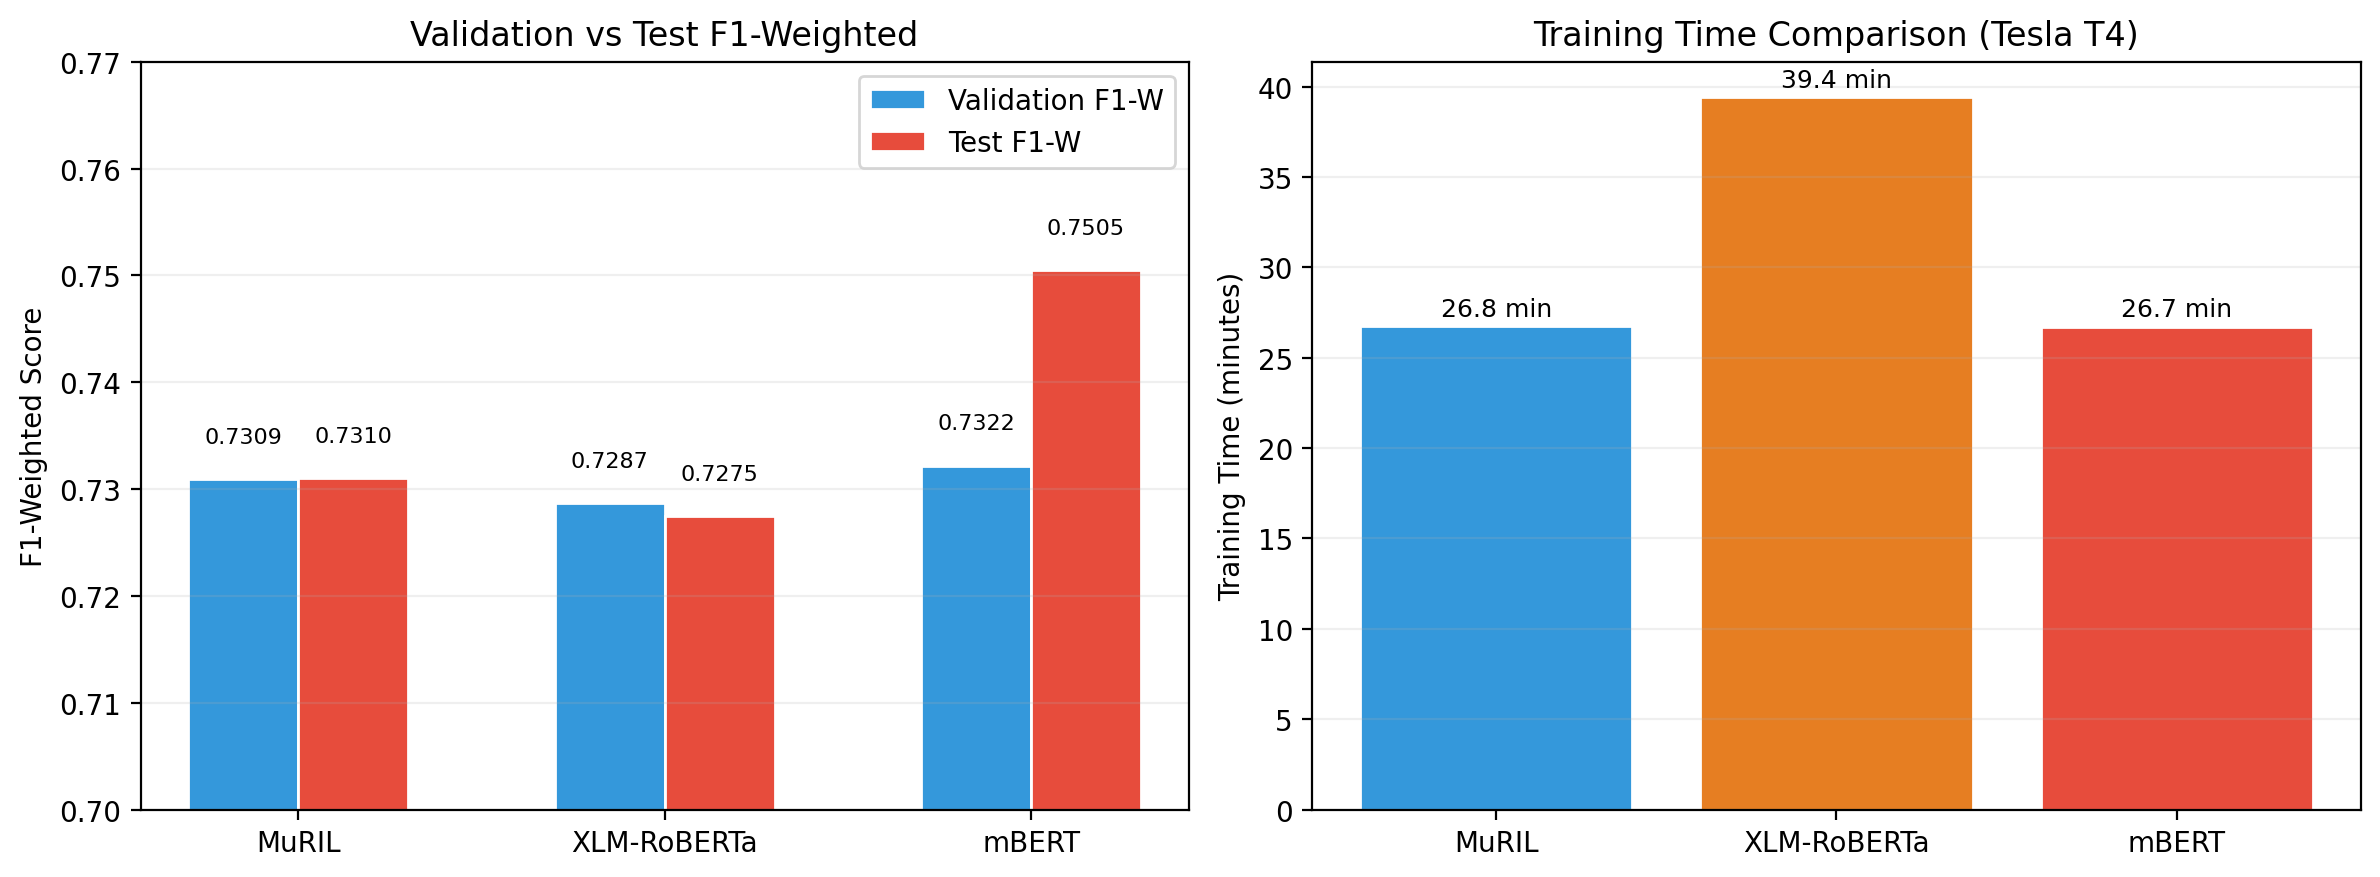
\includegraphics[width=0.98\columnwidth]{figures/training_analysis.png}
\caption{Left: Validation vs.\ test F1-W showing the gap for MuRIL. Right: Training time comparison on Tesla T4 GPU.}
\label{fig:training_analysis}
\end{figure}

\begin{figure}[!t]
\centering
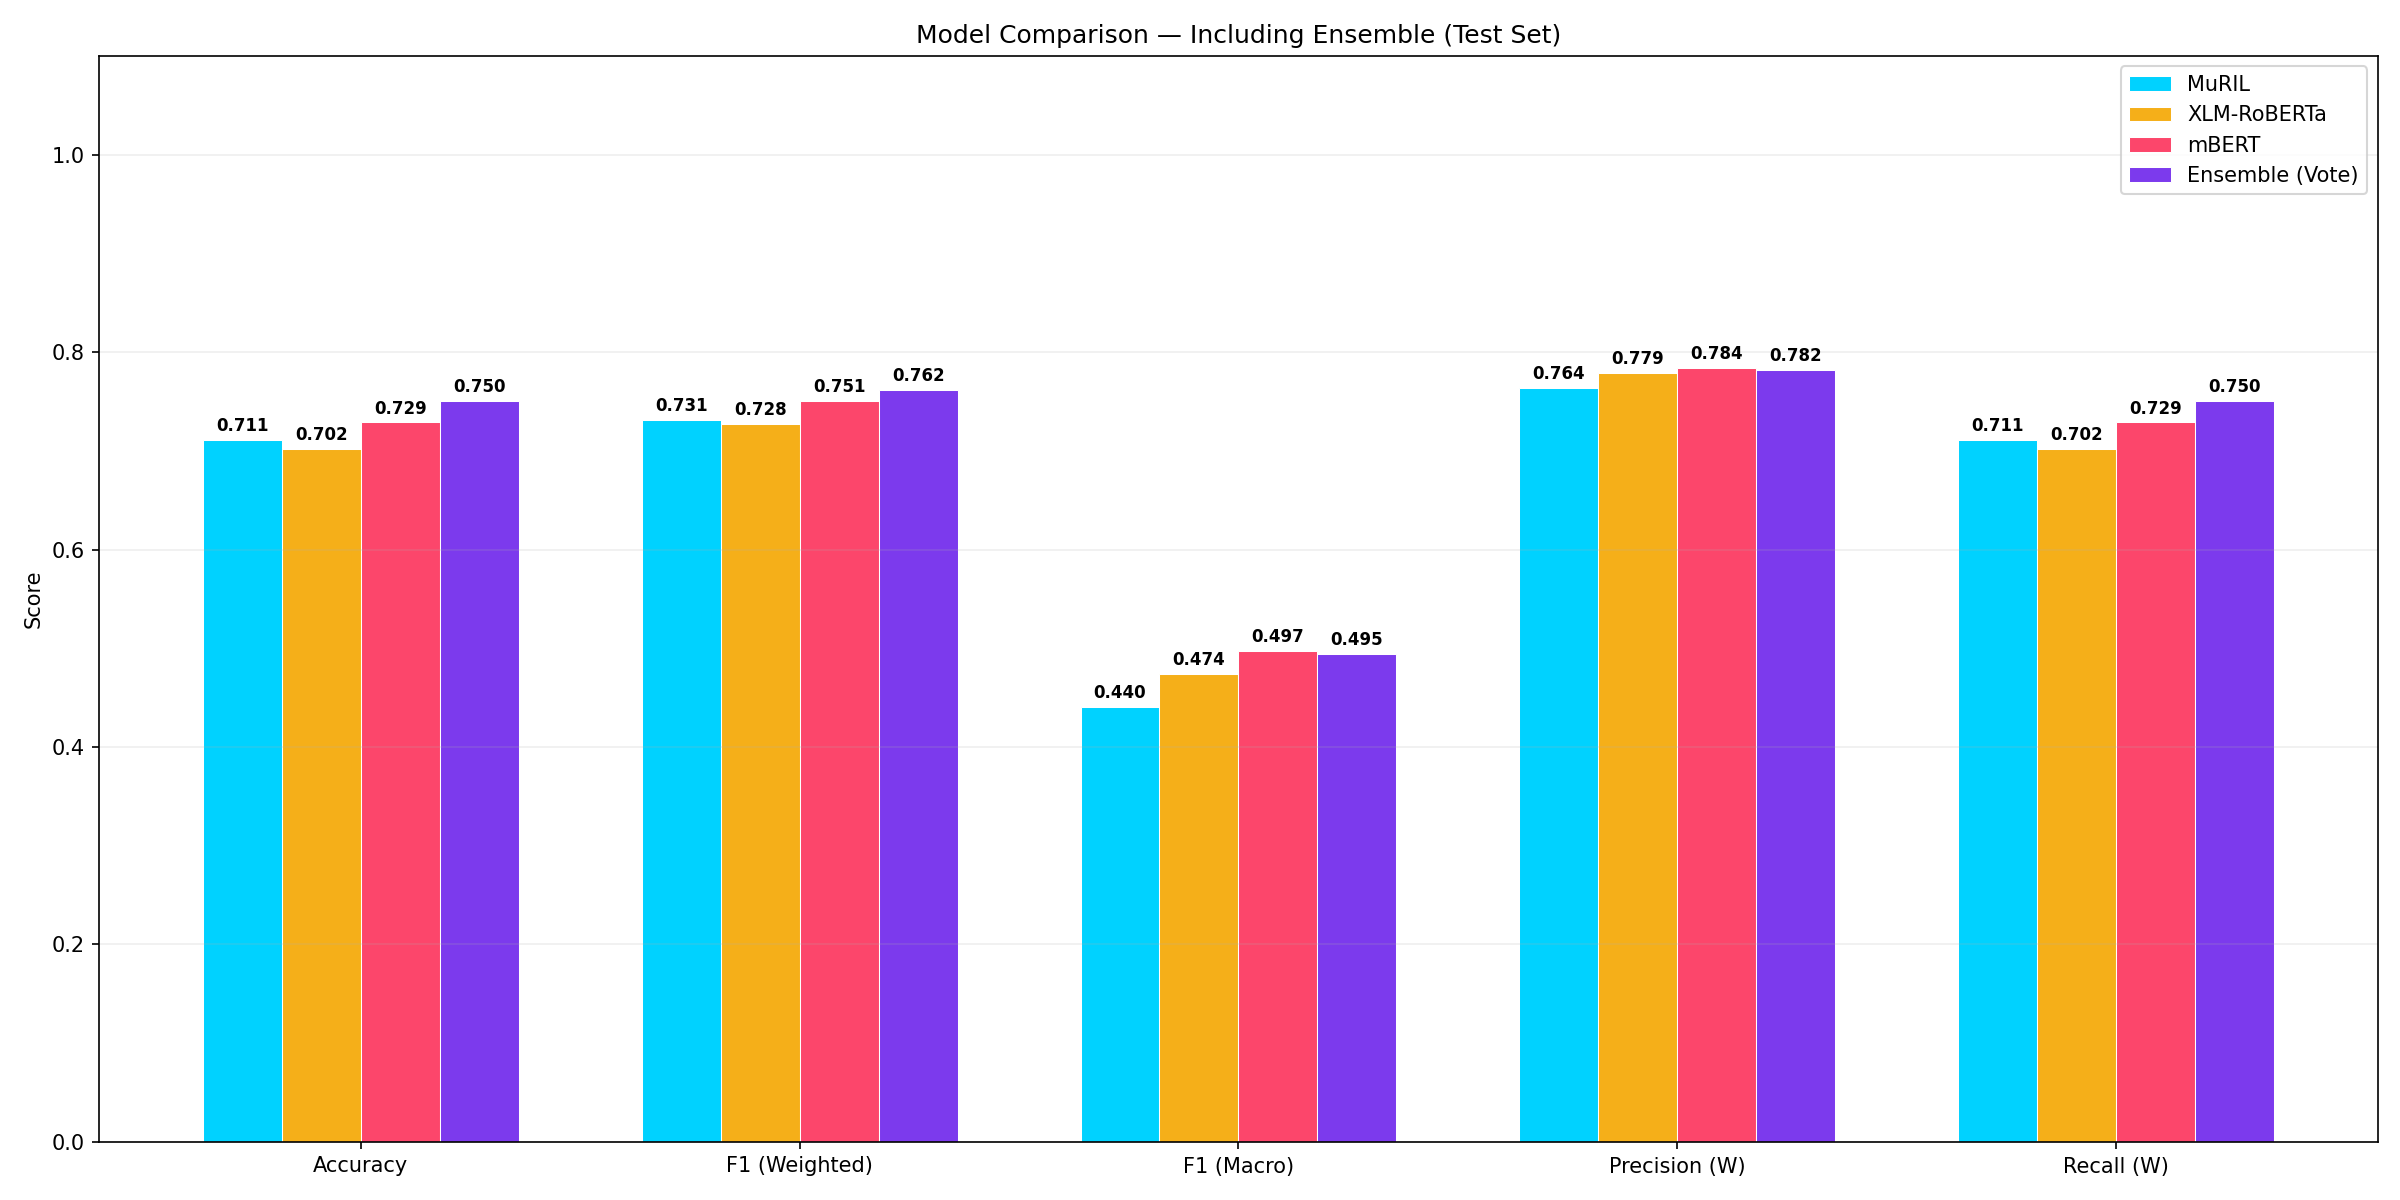
\includegraphics[width=0.98\columnwidth]{figures/model_comparison_with_ensemble.png}
\caption{Comparison of evaluation metrics across all models and ensemble.}
\label{fig:model_comparison}
\end{figure}

\subsection{Comparison with Shared Task Systems}

\begin{table}[!t]
\centering
\caption{Context: DravidianLangTech-2021 Shared Task (Different Test Set)}
\label{tab:baselines}
\begin{tabular}{lcc}
\toprule
\textbf{System} & \textbf{F1-W} & \textbf{Test Set} \\
\midrule
hate-alert (1st) \cite{chakravarthi2021dravidian} & 0.78$^\dagger$ & Official \\
Top-5 range \cite{chakravarthi2021dravidian} & 0.75--0.78$^\dagger$ & Official \\
Median participant \cite{chakravarthi2021dravidian} & $\approx$0.70$^\dagger$ & Official \\
\midrule
mBERT (ours) & 0.7505 & Custom split \\
Ensemble (ours) & 0.7620 & Custom split \\
\bottomrule
\multicolumn{3}{l}{\footnotesize $^\dagger$ Tested on official test set; not directly comparable.}
\end{tabular}
\end{table}

Table~\ref{tab:baselines} provides approximate context against DravidianLangTech-2021 shared task scores. \textbf{Caveat:} Direct comparison is not valid as we use a different test split. Our ensemble F1-W of 0.7620 falls within the competitive range.

\subsection{Performance by Script Type}

\begin{table}[!t]
\centering
\caption{F1-Weighted by Script Type on Test Set}
\label{tab:script_perf}
\begin{tabular}{lrcccc}
\toprule
\textbf{Script} & \textbf{N} & \textbf{MuRIL} & \textbf{XLM-R} & \textbf{mBERT} & \textbf{Ens.} \\
\midrule
Latin & 1762 & 0.719 & 0.717 & 0.749 & \textbf{0.756} \\
Tamil & 416 & \textbf{0.771} & 0.758 & 0.747 & \textbf{0.775} \\
Mixed & 12 & 0.741 & 0.782 & 0.796 & \textbf{0.845} \\
\bottomrule
\end{tabular}
\end{table}

Table~\ref{tab:script_perf} reveals a key finding: \textbf{MuRIL outperforms all other individual models on pure Tamil Unicode text} (F1-W: 0.771 vs.\ mBERT's 0.747), confirming that Indian-language-specific pre-training provides advantages for native-script content. However, mBERT dominates on Latin/Tanglish text (0.749 vs.\ 0.719), which constitutes 80\% of the test set, explaining its overall superiority. The ensemble achieves the best performance across all script types.

\subsection{Per-Class Performance}

\begin{table}[!t]
\centering
\caption{Per-Class F1 Scores}
\label{tab:perclass}
\begin{tabular}{lcccc}
\toprule
\textbf{Class} & \textbf{MuRIL} & \textbf{XLM-R} & \textbf{mBERT} & \textbf{Ens.} \\
\midrule
Not\_offensive & 0.863 & 0.835 & 0.863 & \textbf{0.876} \\
Off\_Untargeted & 0.383 & 0.411 & 0.405 & \textbf{0.430} \\
Off\_Targ\_Indiv & 0.230 & 0.421 & \textbf{0.445} & 0.425 \\
Off\_Targ\_Group & 0.321 & 0.362 & 0.360 & \textbf{0.377} \\
Off\_Targ\_Other & 0.000 & 0.000 & \textbf{0.082} & 0.000 \\
not-Tamil & 0.846 & 0.817 & 0.828 & \textbf{0.860} \\
\bottomrule
\end{tabular}
\end{table}

The ensemble wins on 4 of 6 classes (Table~\ref{tab:perclass}). The \texttt{Offensive\_Targeted\_Other} class (30 test samples) remains effectively undetectable across all approaches.

\subsection{Confusion Matrix Analysis}

\begin{figure}[!t]
\centering
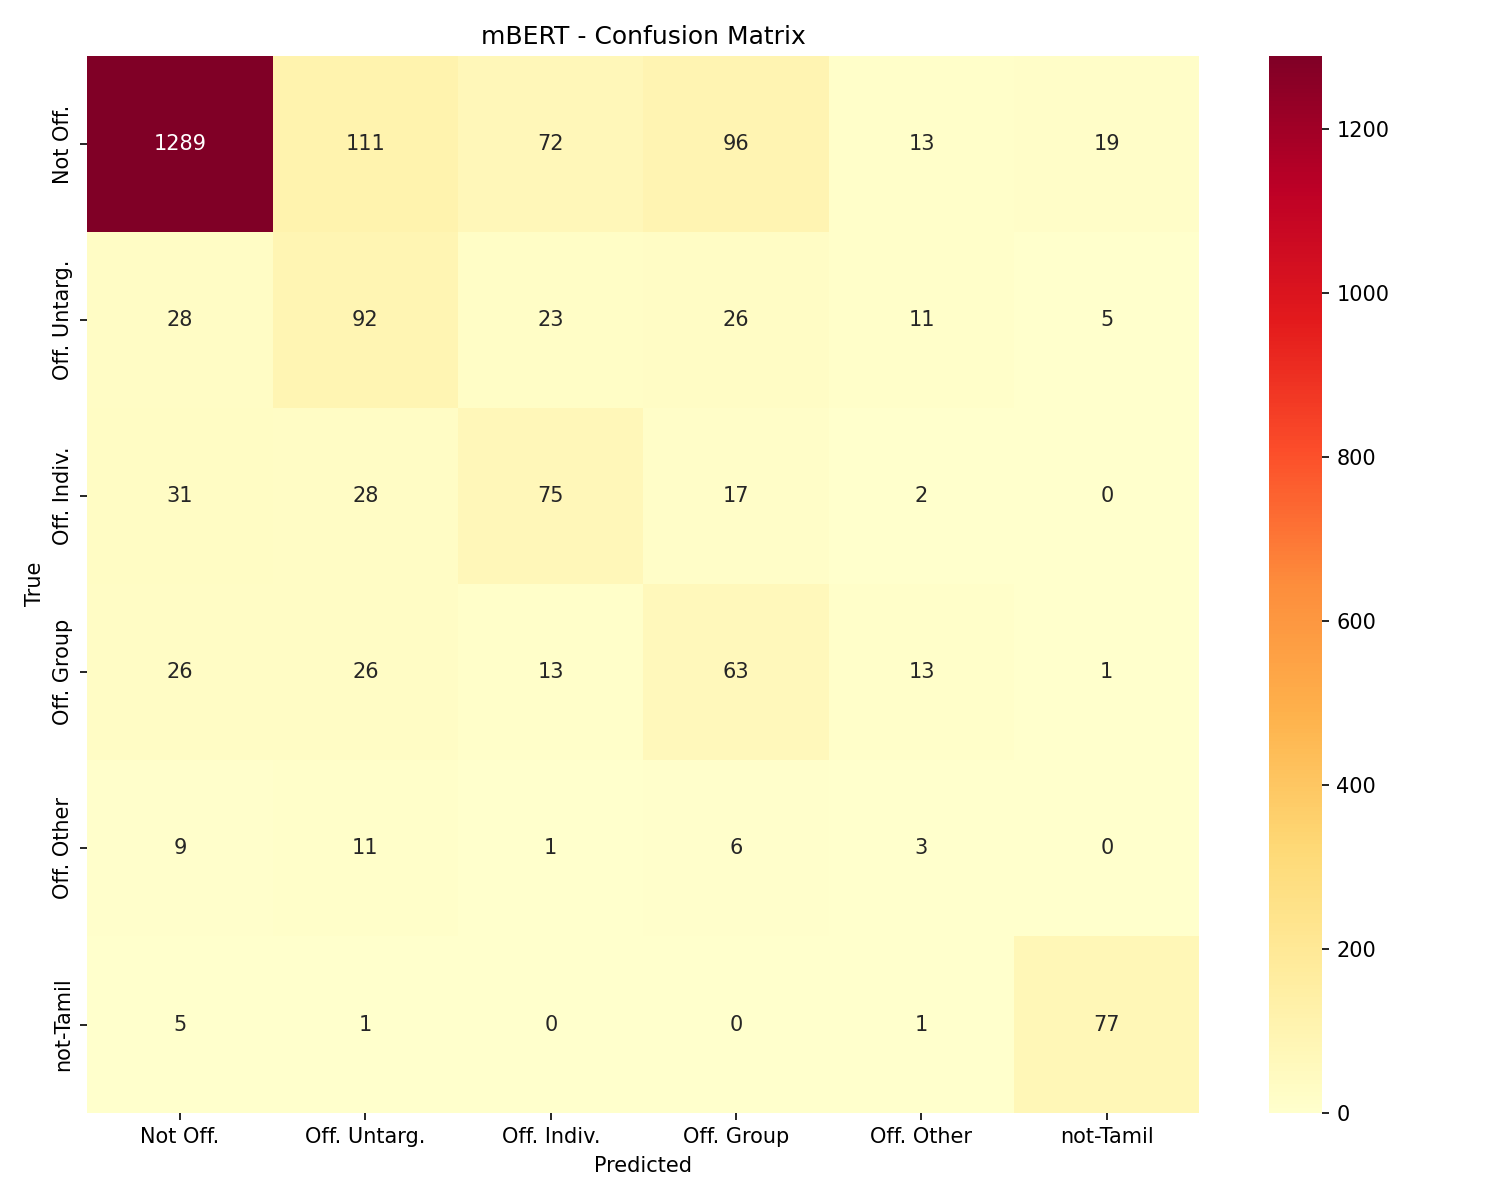
\includegraphics[width=0.95\columnwidth]{figures/mbert_confusion_matrix.png}
\caption{Confusion matrix for mBERT on the test set.}
\label{fig:cm_mbert}
\end{figure}

\begin{figure}[!t]
\centering
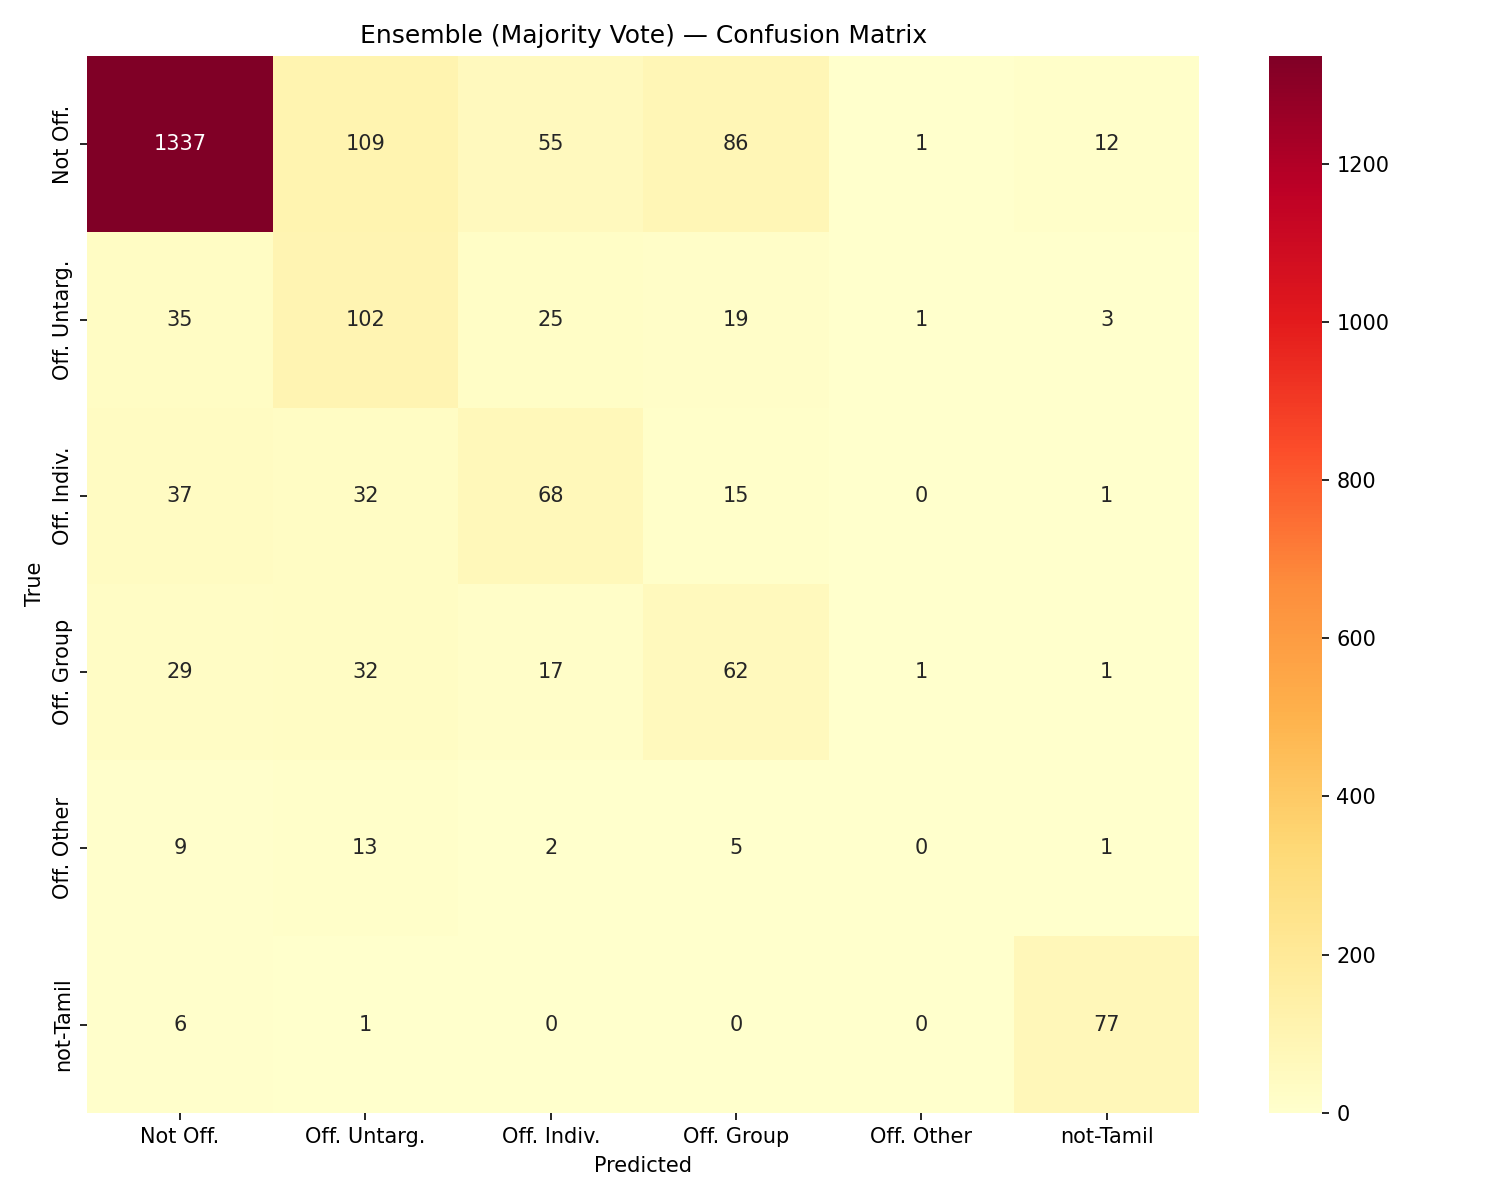
\includegraphics[width=0.95\columnwidth]{figures/ensemble_confusion_matrix.png}
\caption{Confusion matrix for the ensemble on the test set.}
\label{fig:cm_ensemble}
\end{figure}

Key observations from the confusion matrices (Figs.~\ref{fig:cm_mbert}--\ref{fig:cm_ensemble}):
\begin{enumerate}
    \item Strong majority-class detection (Not\_offensive F1 $>$ 0.83).
    \item Significant confusion between \texttt{Off\_Untargeted} and \texttt{Off\_Targeted\_Group}, likely due to overlapping caste discourse.
    \item Reliable language identification for \texttt{not-Tamil} (F1 $>$ 0.81).
\end{enumerate}

%=====================================================
\section{Error Analysis and Explainability}
%=====================================================

\subsection{Error Categorization}

We categorize the 595 errors from mBERT (27.1\% error rate):

\begin{enumerate}
    \item \textbf{False Positives (292 cases, 49.1\%)}: Non-offensive text flagged as offensive --- the largest category. Aggressive fan discourse and caste-community solidarity messages are frequently misclassified.
    \item \textbf{Dangerous False Negatives (94 cases, 15.8\%)}: Offensive text escaping detection --- critical for content moderation.
    \item \textbf{Cross-Category (159 cases, 26.7\%)}: Confusion between offensive sub-types.
    \item \textbf{not-Tamil Errors (50 cases, 8.4\%)}: Hindi/Telugu comments misidentified.
\end{enumerate}

\subsection{LIME Explainability Analysis}

We use LIME \cite{ribeiro2016lime} to generate word-level feature attributions for mBERT predictions on representative samples. Fig.~\ref{fig:lime} presents three examples.

\begin{figure*}[!t]
\centering
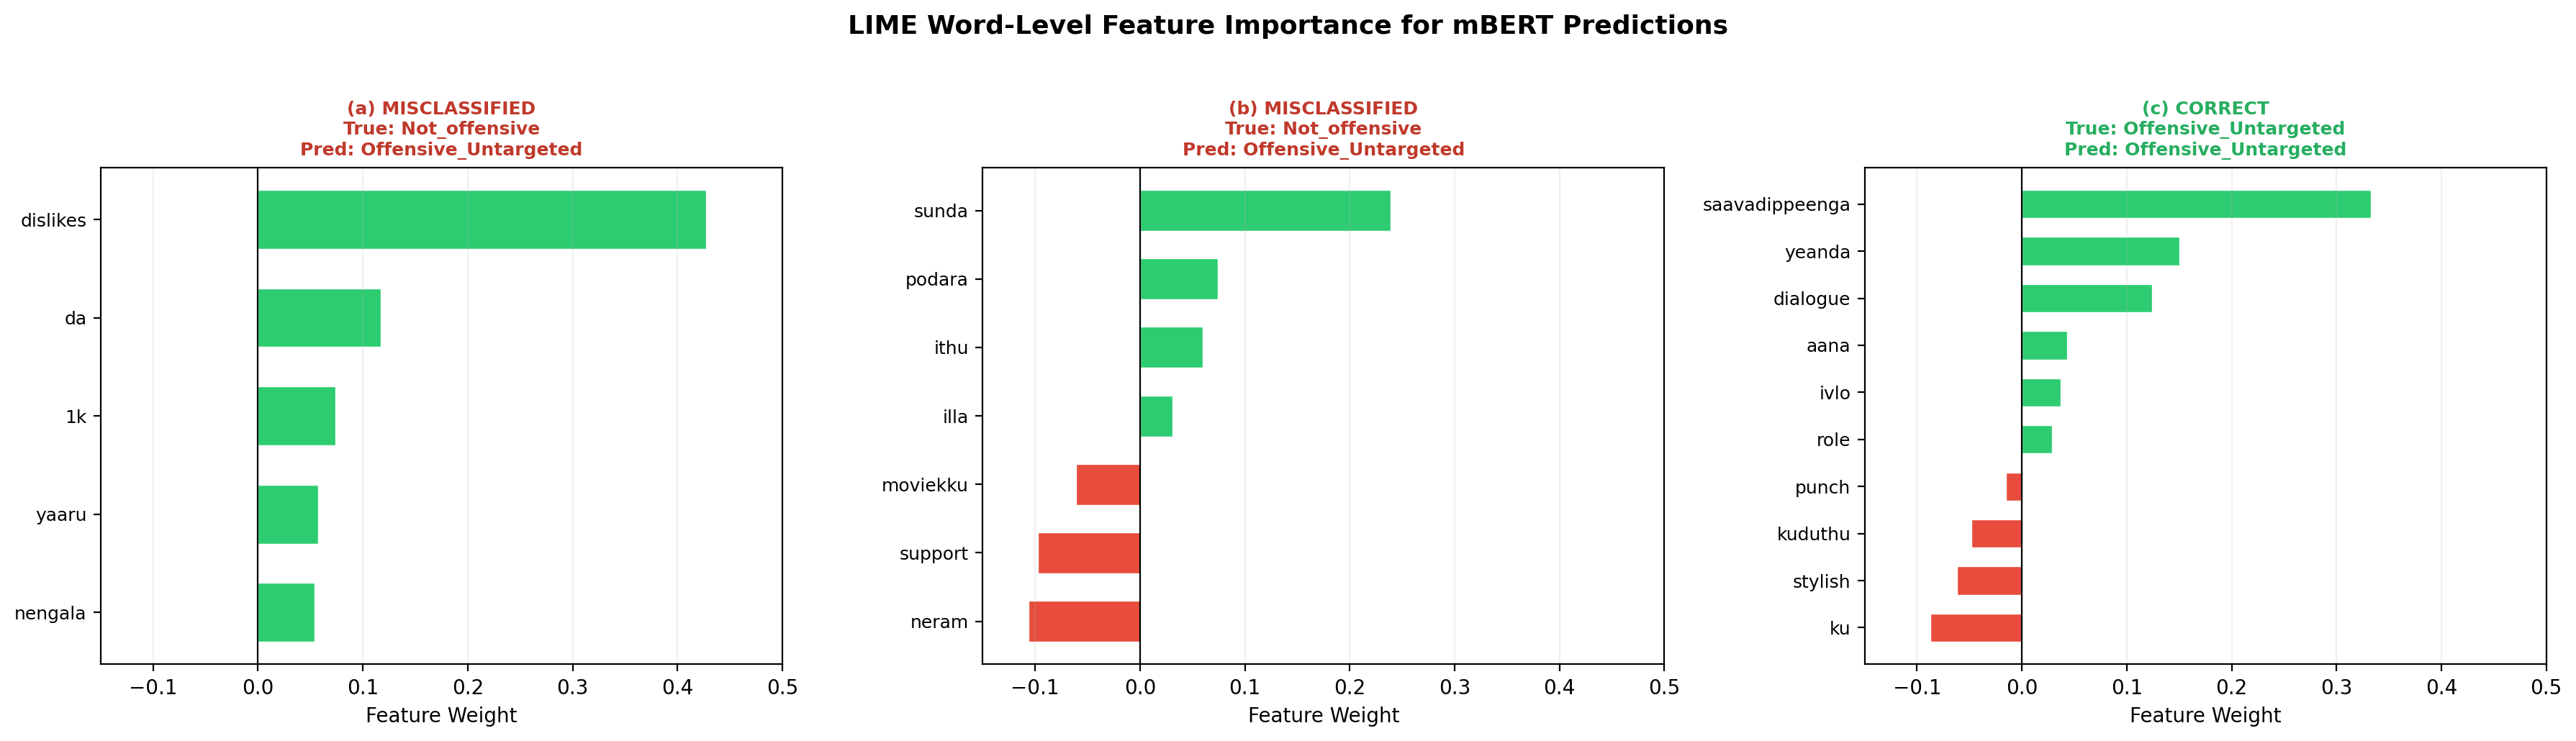
\includegraphics[width=0.92\textwidth]{figures/lime_explanations.png}
\caption{LIME word-level feature importance for three mBERT predictions. Green bars indicate features pushing toward the predicted class; red bars push against it. (a, b) Misclassified samples where aggressive-sounding but non-offensive words (``dislikes'', ``sunda'') trigger false positive predictions. (c) Correctly classified offensive sample where Tamil profanity (``saavadippeenga'') is the dominant feature.}
\label{fig:lime}
\end{figure*}

Key findings from LIME analysis:

\begin{enumerate}
    \item \textbf{Legitimate offensive cues}: Tamil profanity (e.g., ``saavadippeenga'' = roughly ``you'll be killed'') correctly receives high positive weight (0.333), driving accurate offensive predictions (Fig.~\ref{fig:lime}c).
    \item \textbf{Spurious correlations}: The word ``dislikes'' receives the highest weight (0.427) in a non-offensive context about YouTube metrics, triggering a false positive (Fig.~\ref{fig:lime}a). The model appears to associate negative-sentiment English words with offensiveness.
    \item \textbf{Context-dependent aggression}: The word ``sunda'' (colloquial for ``nothing/useless'') triggers offensive prediction (0.239) even in a casual, non-offensive comment (Fig.~\ref{fig:lime}b). This reveals the model's inability to distinguish casual Tamil slang from genuine offense.
    \item \textbf{Opposing features}: Words like ``support'' and ``neram'' (time) receive negative weights, correctly pushing away from offensive prediction, but are overridden by stronger spurious signals.
\end{enumerate}

\textbf{Limitation:} This analysis covers only 3 of 8 generated LIME samples due to space constraints. A comprehensive quantitative explainability evaluation (e.g., faithfulness and sufficiency metrics \cite{mathew2021hatexplain}) is planned as future work.

%=====================================================
\section{Discussion}
%=====================================================

\subsection{MuRIL vs.\ General Multilingual Models}

Contrary to our initial hypothesis, MuRIL did not achieve the best \textit{overall} test-set performance despite its Indian-language-specific pre-training (F1-W: 0.7310 vs.\ mBERT's 0.7505). However, the per-script analysis (Table~\ref{tab:script_perf}) reveals a nuanced picture: \textbf{MuRIL is the best individual model on pure Tamil Unicode text} (F1-W: 0.771), confirming that Indian-language pre-training helps for native-script content. Its overall inferiority is driven by weaker Latin/Tanglish performance (0.719 vs.\ 0.749), which dominates the test set (80\%).

This suggests that MuRIL's advantage is script-dependent: strong on formal Tamil but weaker on informal transliterated text, possibly because its transliteration pre-training does not fully capture the creative, non-standard spellings of YouTube Tanglish. \textbf{We caution that this finding is based on a single random seed and a single test split}, and should be validated with multi-seed experiments.

\subsection{Ensemble Trade-offs}

The ensemble improves F1-W (+1.15\%) and accuracy (+2.14\%) but slightly decreases F1-Macro ($-$0.25\%). This is because majority voting inherently favors the majority class: when 2 of 3 models predict Not\_offensive, the ensemble follows, even if the third model correctly identifies a minority-class offensive sample. Weighted or learned ensemble strategies could mitigate this.

\subsection{Challenges}

\begin{enumerate}
    \item \textbf{Class imbalance}: The dominant challenge. Weighted loss alone is insufficient for extreme minority classes ($<$2\% of data).
    \item \textbf{False positive burden}: 292 false positives vs.\ 94 false negatives suggests over-moderation, problematic for user experience.
    \item \textbf{Cultural context}: Caste solidarity messages and fan discourse use aggressive language that is contextually non-offensive but lexically indistinguishable from genuine abuse.
\end{enumerate}

\subsection{Limitations}

\begin{enumerate}
    \item \textbf{Single random seed}: Results may vary with different initializations. Multi-seed experiments with confidence intervals are needed.
    \item \textbf{Custom test split}: Our test set differs from the official shared task test set, limiting direct comparison with published work.
    \item \textbf{Platform specificity}: YouTube comments may not generalize to Twitter/X, WhatsApp, or other platforms.
    \item \textbf{Limited LIME scope}: Only 8 qualitative samples analyzed; quantitative explainability metrics are not reported.
    \item \textbf{Single imbalance strategy}: Only weighted cross-entropy explored; focal loss, oversampling, and two-stage approaches may improve minority-class detection.
\end{enumerate}

%=====================================================
\section{Ethical Considerations}
%=====================================================

This work involves processing offensive and potentially harmful content, including caste-based slurs and targeted abuse. We acknowledge the following ethical dimensions:

\begin{enumerate}
    \item \textbf{Annotator welfare}: The dataset was created by external researchers \cite{chakravarthi2021dataset}; we did not perform annotation. Exposure to offensive content can cause psychological harm to annotators.
    \item \textbf{Dual use}: Automated offensive language detection systems can be misused for censorship or suppression of legitimate speech, particularly in politically sensitive contexts.
    \item \textbf{Bias amplification}: The model inherits biases from training data. The high false positive rate on caste-community messages suggests the model may disproportionately flag content from certain communities.
    \item \textbf{Cultural sensitivity}: Offensiveness is culturally and contextually dependent. Models trained on Tamil YouTube data should not be deployed for other Tamil-speaking contexts without re-evaluation.
\end{enumerate}

%=====================================================
\section{Conclusion and Future Work}
%=====================================================

This paper presents a comparative study of multilingual transformers for Tamil offensive language detection. Our experiments demonstrate that mBERT achieves the best individual F1-W of 0.7505, and a majority-voting ensemble improves this to 0.7620, competitive with DravidianLangTech-2021 shared task systems. Contrary to expectations, MuRIL did not outperform general multilingual models on this code-mixed dataset.

Key takeaways:
\begin{enumerate}
    \item General multilingual pre-training can be equally effective as Indian-language-specific pre-training for informal, code-mixed text.
    \item Majority-voting ensemble improves F1-W but slightly hurts F1-Macro due to majority-class bias.
    \item LIME analysis reveals spurious correlations with negative-sentiment English words and context-insensitive slang detection.
    \item Class imbalance remains the dominant challenge for minority offensive sub-types.
\end{enumerate}

\textbf{Future Work.} We plan to (1) conduct multi-seed experiments with bootstrap confidence intervals, (2) explore focal loss and oversampling strategies, (3) extend to other Dravidian languages, (4) implement learned ensemble methods, and (5) develop quantitative explainability benchmarks.

\textbf{Code and Data Availability.} Our code is available at \url{https://github.com/naveen-231006/Hate-Word}. The OffensEval Dravidian dataset is publicly available via HuggingFace Datasets \cite{chakravarthi2021dataset}.

%=====================================================
% REFERENCES
%=====================================================

\begin{thebibliography}{19}

\bibitem{iamai2025}
Internet and Mobile Association of India, ``India Internet Report 2025,'' IAMAI, 2025.

\bibitem{fortuna2018survey}
P.~Fortuna and S.~Nunes, ``A survey on automatic detection of hate speech in text,'' \textit{ACM Computing Surveys}, vol.~51, no.~4, pp.~1--30, 2018.

\bibitem{khanuja2021muril}
S.~Khanuja \textit{et al.}, ``MuRIL: Multilingual Representations for Indian Languages,'' in \textit{Findings of ACL}, 2021, pp.~3929--3936.

\bibitem{conneau2020xlmr}
A.~Conneau \textit{et al.}, ``Unsupervised cross-lingual representation learning at scale,'' in \textit{Proc. ACL}, 2020, pp.~8440--8451.

\bibitem{devlin2019bert}
J.~Devlin \textit{et al.}, ``BERT: Pre-training of deep bidirectional transformers for language understanding,'' in \textit{Proc. NAACL-HLT}, 2019, pp.~4171--4186.

\bibitem{davidson2017automated}
T.~Davidson, D.~Warmsley, M.~Macy, and I.~Weber, ``Automated hate speech detection and the problem of offensive language,'' in \textit{Proc. ICWSM}, 2017, pp.~512--515.

\bibitem{waseem2016hateful}
Z.~Waseem and D.~Hovy, ``Hateful symbols or hateful people? Predictive features for hate speech detection on Twitter,'' in \textit{Proc. NAACL Student Research Workshop}, 2016, pp.~88--93.

\bibitem{badjatiya2017deep}
P.~Badjatiya \textit{et al.}, ``Deep learning for hate speech detection in tweets,'' in \textit{Proc. WWW Companion}, 2017, pp.~759--760.

\bibitem{caselli2021hatebert}
T.~Caselli \textit{et al.}, ``HateBERT: Retraining BERT for abusive language detection in English,'' in \textit{Proc. WOAH}, 2021, pp.~17--25.

\bibitem{pamungkas2019cross}
M.~Pamungkas and V.~Patti, ``Cross-domain and cross-lingual abusive language detection,'' in \textit{Proc. ACL Student Research Workshop}, 2019, pp.~363--370.

\bibitem{chakravarthi2021dravidian}
B.~R.~Chakravarthi \textit{et al.}, ``Findings of the shared task on offensive language identification in Tamil, Malayalam, and Kannada,'' in \textit{Proc. DravidianLangTech, EACL}, 2021.

\bibitem{chakravarthi2021dataset}
B.~R.~Chakravarthi \textit{et al.}, ``Dataset for identification of homophobia and transphobia in multilingual YouTube comments,'' \textit{arXiv preprint arXiv:2109.00227}, 2021.

\bibitem{dowlagar2021cfilt}
S.~Dowlagar and R.~Mamidi, ``CfiltIITB at DravidianLangTech@EACL2021,'' in \textit{Proc. EACL Workshop}, 2021.

\bibitem{risch2020data}
J.~Risch \textit{et al.}, ``Data augmentation for cross-domain hate speech detection,'' \textit{arXiv preprint arXiv:2004.10404}, 2020.

\bibitem{rajamanickam2020joint}
V.~Rajamanickam \textit{et al.}, ``Joint multitask learning for community question answering,'' in \textit{Proc. EMNLP}, 2020.

\bibitem{ribeiro2016lime}
M.~T.~Ribeiro \textit{et al.}, ``Why should I trust you?: Explaining the predictions of any classifier,'' in \textit{Proc. KDD}, 2016, pp.~1135--1144.

\bibitem{lundberg2017shap}
S.~M.~Lundberg and S.~Lee, ``A unified approach to interpreting model predictions,'' in \textit{Proc. NeurIPS}, 2017, pp.~4765--4774.

\bibitem{mathew2021hatexplain}
A.~Mathew \textit{et al.}, ``HateXplain: A benchmark dataset for explainable hate speech detection,'' in \textit{Proc. AAAI}, 2021, pp.~14867--14875.

\end{thebibliography}

\end{document}
